
%%%%%%%%%%%%%%%%%%%%%%%%%%%%%%%%%%%%%%%%%
% Short Sectioned Assignment LaTeX Template Version 1.0 (5/5/12)
% This template has been downloaded from: http://www.LaTeXTemplates.com
% Original author:  Frits Wenneker (http://www.howtotex.com)
% License: CC BY-NC-SA 3.0 (http://creativecommons.org/licenses/by-nc-sa/3.0/)
%%%%%%%%%%%%%%%%%%%%%%%%%%%%%%%%%%%%%%%%%

%----------------------------------------------------------------------------------------
%	PACKAGES AND OTHER DOCUMENT CONFIGURATIONS
%----------------------------------------------------------------------------------------

\documentclass[paper=a4, fontsize=11pt]{scrartcl} % A4 paper and 11pt font size

% ---- Entrada y salida de texto -----

\usepackage[T1]{fontenc} % Use 8-bit encoding that has 256 glyphs
\usepackage[utf8]{inputenc}
%\usepackage{fourier} % Use the Adobe Utopia font for the document - comment this line to return to the LaTeX default

% ---- Idioma --------

\usepackage[spanish, es-tabla]{babel} % Selecciona el español para palabras introducidas automáticamente, p.ej. "septiembre" en la fecha y especifica que se use la palabra Tabla en vez de Cuadro

% ---- Otros paquetes ----

\usepackage{url} % ,href} %para incluir URLs e hipervínculos dentro del texto (aunque hay que instalar href)
\usepackage{amsmath,amsfonts,amsthm} % Math packages
%\usepackage{graphics,graphicx, floatrow} %para incluir imágenes y notas en las imágenes
\usepackage{graphics,graphicx, float} %para incluir imágenes y colocarlas
\usepackage{movie15}

% Para hacer tablas comlejas
%\usepackage{multirow}
%\usepackage{threeparttable}

%\usepackage{sectsty} % Allows customizing section commands
%\allsectionsfont{\centering \normalfont\scshape} % Make all sections centered, the default font and small caps

\usepackage{fancyhdr} % Custom headers and footers

\pagestyle{fancyplain} % Makes all pages in the document conform to the custom headers and footers
\fancyhead{} % No page header - if you want one, create it in the same way as the footers below
\fancyfoot[L]{} % Empty left footer
\fancyfoot[C]{} % Empty center footer
\fancyfoot[R]{\thepage} % Page numbering for right footer
\renewcommand{\headrulewidth}{0pt} % Remove header underlines
\renewcommand{\footrulewidth}{0pt} % Remove footer underlines
\setlength{\headheight}{13.6pt} % Customize the height of the header

\numberwithin{equation}{section} % Number equations within sections (i.e. 1.1, 1.2, 2.1, 2.2 instead of 1, 2, 3, 4)
\numberwithin{figure}{section} % Number figures within sections (i.e. 1.1, 1.2, 2.1, 2.2 instead of 1, 2, 3, 4)
\numberwithin{table}{section} % Number tables within sections (i.e. 1.1, 1.2, 2.1, 2.2 instead of 1, 2, 3, 4)

\setlength\parindent{0pt} % Removes all indentation from paragraphs - comment this line for an assignment with lots of text

\newcommand{\horrule}[1]{\rule{\linewidth}{#1}} % Create horizontal rule command with 1 argument of height
\usepackage[breaklinks=true]{hyperref}
\usepackage{bookmark}
\usepackage{wasysym}
\usepackage{subcaption}
\usepackage[dvipsnames]{xcolor}
\usepackage{amssymb}
\usepackage{color}
\usepackage{listings}
\usepackage{upgreek} % para poner letras griegas sin cursiva
\usepackage{cancel} % para tachar
\usepackage{mathdots} % para el comando \iddots
\usepackage{mathrsfs} % para formato de letra
\usepackage{stackrel} % para el comando \stackbin
\lstdefinestyle{cmas}
{ %
	language=C++,                % elegir el lenguaje del código
	stringstyle=\color{blue}\ttfamily,,
	basicstyle=\normalsize\ttfamily,       % el tamaño del font a usar para el código
	numbers=left,                   % dónde poner los números de línea 
	numberstyle=\footnotesize,      % tamaño de font usados para los números de línea 
	stepnumber=1,                   % el paso de numeración
	numbersep=8pt,                  % distancia del numero de línea y la línea
	backgroundcolor=\color{white},  % color de fondo, para usarlo hay que agregar  \usepackage{color}
	showspaces=false,               % mostrar espacios en blanco ?
	showstringspaces=false,         % subrayar espacios con cadenas?   
	 showtabs=false,                 % mostrar taba usando cadenas? 
	frame=single,           			% enmarcar el código?  
	tabsize=2,          				% sets default tabsize to 2 spaces?
	keywordstyle=\color{MidnightBlue}\ttfamily\bfseries,
	commentstyle=\color{OliveGreen}\ttfamily,
	morecomment=[l][\color{OliveGreen}]{\#},
	captionpos=b,           % sets the caption-position to bottom?
	breaklines=true,        % sets automatic line breaking?
	breakatwhitespace=false,    % sets if automatic breaks should only happen at whitespace ?
	title=\lstname,
	escapeinside={\%*}{*)}          % if you want to add a comment within your code
}

\lstdefinestyle{payt}
{ %
	language=Python,                % elegir el lenguaje del código
	stringstyle=\color{blue}\ttfamily,,
	basicstyle=\normalsize\ttfamily,       % el tamaño del font a usar para el código
	numbers=left,                   % dónde poner los números de línea 
	numberstyle=\footnotesize,      % tamaño de font usados para los números de línea 
	stepnumber=1,                   % el paso de numeración
	numbersep=8pt,                  % distancia del numero de línea y la línea
	backgroundcolor=\color{white},  % color de fondo, para usarlo hay que agregar  \usepackage{color}
	showspaces=false,               % mostrar espacios en blanco ?
	showstringspaces=false,         % subrayar espacios con cadenas?   
	showtabs=false,                 % mostrar taba usando cadenas? 
	frame=single,           			% enmarcar el código?  
	tabsize=2,          				% sets default tabsize to 2 spaces?
	keywordstyle=\color{MidnightBlue}\ttfamily\bfseries,
	commentstyle=\color{OliveGreen}\ttfamily,
	morecomment=[l][\color{OliveGreen}]{\#},
	captionpos=b,           % sets the caption-position to bottom?
	breaklines=true,        % sets automatic line breaking?
	breakatwhitespace=false,    % sets if automatic breaks should only happen at whitespace ?
	title=\lstname,
	escapeinside={\%*}{*)}          % if you want to add a comment within your code
}

\definecolor{light-gray}{gray}{0.85}

\lstdefinestyle{fich}
{ %
	language=Bash,                % elegir el lenguaje del código
	stringstyle=\color{black}\texttt,
	basicstyle=\normalsize\ttfamily,       % el tamaño del font a usar para el código	
	numbers=left,                   % dónde poner los números de línea 
	numberstyle=\footnotesize,      % tamaño de font usados para los números de línea 
	stepnumber=1,                   % el paso de numeración
	numbersep=8pt,                  % distancia del numero de línea y la línea
	backgroundcolor=\color{light-gray},  % color de fondo, para usarlo hay que agregar  \usepackage{color}
	showspaces=false,               % mostrar espacios en blanco ?
	showstringspaces=false,         % subrayar espacios con cadenas?   
	showtabs=false,                 % mostrar taba usando cadenas? 
%	frame=single,           			% enmarcar el código?  
	tabsize=2,          				% sets default tabsize to 2 spaces?
	captionpos=b,           % sets the caption-position to bottom?
	breaklines=true,        % sets automatic line breaking?
	breakatwhitespace=false,    % sets if automatic breaks should only happen at whitespace ?
	title=\lstname,
	escapeinside={\%*}{*)}          % if you want to add a comment within your code
}

\lstset{literate=
  {á}{{\'a}}1 {é}{{\'e}}1 {í}{{\'i}}1 {ó}{{\'o}}1 {ú}{{\'u}}1
  {Á}{{\'A}}1 {É}{{\'E}}1 {Í}{{\'I}}1 {Ó}{{\'O}}1 {Ú}{{\'U}}1
  {à}{{\`a}}1 {è}{{\`e}}1 {ì}{{\`i}}1 {ò}{{\`o}}1 {ù}{{\`u}}1
  {À}{{\`A}}1 {È}{{\'E}}1 {Ì}{{\`I}}1 {Ò}{{\`O}}1 {Ù}{{\`U}}1
  {ä}{{\"a}}1 {ë}{{\"e}}1 {ï}{{\"i}}1 {ö}{{\"o}}1 {ü}{{\"u}}1
  {Ä}{{\"A}}1 {Ë}{{\"E}}1 {Ï}{{\"I}}1 {Ö}{{\"O}}1 {Ü}{{\"U}}1
  {â}{{\^a}}1 {ê}{{\^e}}1 {î}{{\^i}}1 {ô}{{\^o}}1 {û}{{\^u}}1
  {Â}{{\^A}}1 {Ê}{{\^E}}1 {Î}{{\^I}}1 {Ô}{{\^O}}1 {Û}{{\^U}}1
  {œ}{{\oe}}1 {Œ}{{\OE}}1 {æ}{{\ae}}1 {Æ}{{\AE}}1 {ß}{{\ss}}1
  {ű}{{\H{u}}}1 {Ű}{{\H{U}}}1 {ő}{{\H{o}}}1 {Ő}{{\H{O}}}1
  {ç}{{\c c}}1 {Ç}{{\c C}}1 {ø}{{\o}}1 {å}{{\r a}}1 {Å}{{\r A}}1
  {€}{{\EUR}}1 {£}{{\pounds}}1
  {ñ}{{\~n}}1
}

\hypersetup{
    colorlinks=true,
    linkcolor=black,
    filecolor=magenta,      
    urlcolor=blue,
    pdftitle={ISE: Práctica 3 - Mario Rodríguez Ruiz},
    bookmarks=true,
    citecolor=blue,
}



%----------------------------------------------------------------------------------------
%	TÍTULO Y DATOS DEL ALUMNO
%----------------------------------------------------------------------------------------

\title{	
\normalfont \normalsize 
\textsc{\textbf{Ingeniería de Servidores (2016-2017)} \\ Subgrupo A1 \\ Grado en Ingeniería Informática\\ Universidad de Granada} \\ [25pt] % Your university, school and/or department name(s)
\horrule{0.5pt} \\[0.4cm] % Thin top horizontal rule
\huge Práctica 3: Monitorización de servicios \\ % The assignment title
\horrule{2pt} \\[0.5cm] % Thick bottom horizontal rule
}

\author{Mario Rodríguez Ruiz} % Nombre y apellidos

\date{\normalsize\today} % Incluye la fecha actual

%----------------------------------------------------------------------------------------
% DOCUMENTO
%----------------------------------------------------------------------------------------

\begin{document}

\maketitle % Muestra el Título

\newpage %inserta un salto de página

\tableofcontents % para generar el índice de contenidos

\listoffigures

\newpage

%----------------------------------------------------------------------------------------
%	Cuestión 1
%----------------------------------------------------------------------------------------

\section{Cuestión 1}
\subsection{¿Qué archivo le permite ver qué programas se han
	instalado con el gestor de paquetes?}

El archivo que permite ver qué programas se han instalado con el gestor de paquetes en CentOS es \textbf{/var/log/yum.log} \cite{enlace1}

En la Figura \ref{fig:figura1} se muestra el contenido actual de este fichero en la máquina CentOS.
\begin{figure}[H] %con el [H] le obligamos a situar aquí la figura
	\centering
	\includegraphics[scale=0.9]{figuras/figura1.png} 
	\caption{Contenido del fichero \textbf{/var/log/yum.log} en CentOS} 
	\label{fig:figura1}
\end{figure}

\subsection{¿Qué significan las terminaciones .
	1.gz o .2.gz de los archivos en ese directorio?}
	
Las terminaciones \textbf{1.gz o .2.gz} de los archivos en ese directorio significan que están comprimidos. 

Se trata de ficheros log antiguos: como los logs van creciendo, el sistema los comprime y les aplica una rotación, 
poniéndole la extensión anteriormente nombrada según la antigüedad y creando uno nuevo vacío. \cite{enlace2}
De esta forma se evita que el almacenamiento sea desbordado a causa de los logs.
\\

La utilidad que se encarga de realizar este proceso a diario es \textbf{logrotate}, cuya funcionalidad puede ser personalizada desde su fichero de configuración \textbf{/etc/logrotate.conf} que puede verse en la en la Figura \ref{fig:figura2}

\begin{figure}[H] %con el [H] le obligamos a situar aquí la figura
	\centering
	\includegraphics[scale=0.9]{figuras/figura2.png} 
	\caption{Contenido del fichero \textbf{/etc/logrotate.conf} en CentOS} 
	\label{fig:figura2}
\end{figure}

\newpage

%----------------------------------------------------------------------------------------
%	Cuestión 2
%----------------------------------------------------------------------------------------

\section{Cuestión 2}
\subsection{¿Qué archivo ha de modificar para programar una tarea?}

El archivo que hay que modificar para programar una tarea es \textbf{/etc/crontab} \cite{enlace3} y su contenido actual es el que aparece en la Figura \ref{fig:figura3}

\begin{figure}[H] %con el [H] le obligamos a situar aquí la figura
	\centering
	\includegraphics[scale=0.8]{figuras/figura3.png} 
	\caption{Contenido del fichero \textbf{/etc/crontab} en CentOS} 
	\label{fig:figura3}
\end{figure}

\subsection{Escriba la línea necesaria para ejecutar una vez al día una copia del
	directorio \AC/codigo a \AC{}/seguridad/\$fecha donde \$fecha es la fecha actual
	(puede usar el comando date)}

\begin{lstlisting}[style=fich]
0 8 * * * user cp -r ~/codigo/* ~/seguridad/$(date +%Y%m%d)
\end{lstlisting}

Esta linea realiza la copia del directorio \AC/codigo a \textbf{\AC{}/seguridad/\$fecha}, acción que será ejecutada \textbf{todos los días del año a las 08:00 horas}.

\newpage

%----------------------------------------------------------------------------------------
%	Cuestión 3
%----------------------------------------------------------------------------------------

\section{Cuestión 3}
\subsection{Pruebe a ejecutar el comando, conectar un dispositivo USB y
	vuelva a ejecutar el comando. Copie y pegue la salida del comando.}

La Figura \ref{fig:figura4} muestra la salida del comando \textbf{antes} de la inserción del USB.

\begin{figure}[H] %con el [H] le obligamos a situar aquí la figura
	\centering
	\includegraphics[scale=0.8]{figuras/figura4.png} 
	\caption{Ejecución del comando \textbf{dmesg} antes} 
	\label{fig:figura4}
\end{figure}

La Figura \ref{fig:figura5} muestra la salida del comando \textbf{después} de la inserción del USB.

\begin{figure}[H] %con el [H] le obligamos a situar aquí la figura
	\centering
	\includegraphics[scale=0.8]{figuras/figura5.png} 
	\caption{Ejecución del comando \textbf{dmesg} después} 
	\label{fig:figura5}
\end{figure}

\subsection{Comente qué observa en la información
	mostrada.}

El comando \textbf{dmesg} se ha redirigido a \textbf{tail} para que aparezcan solamente los últimos eventos que se han producido en el sistema.
\\

La información que se muestra en la Figura \ref{fig:figura5} es el vínculo que se ha creado entre el sistema operativo y el USB que se acaba de insertar, así como parte importante de información de éste.
\\

En este caso el SO le ha asignado \textbf{sdc1} al USB, el \textbf{host5} como interfaz SCSI en acceso directo.
Como información, se muestran los bloques de memoria lógica que tiene así como su espacio.

También aparece si tiene la escritura protegida (en este caso no) y el formato del dispositivo (Mode Sense) en el que \textbf{03 00} significa que es un dispositivo de disco \cite{enlace4}. 

Por último, se muestra si dispone de página de modo de caché (no en este caso), cómo asume la memoria cache de la unidad (mediante escritura en este caso) y qué tipo de dispositivo es (disco extraíble adjunto SCSI)

%----------------------------------------------------------------------------------------
%	Cuestión 4
%----------------------------------------------------------------------------------------

\section{Cuestión 4}
\subsection{Ejecute el monitor de $ " $System Performance$ " $ y muestre el
	resultado. Incluya capturas de pantalla comentando la información que
	aparece.}

Para ejecutar el monitor de System Performance una vez dentro del Monitor de rendimento, hay que pulsar \textbf{Iniciar} sobre \textbf{System Performance} dentro de \textbf{Sistema} que aparece en la pestaña \textbf{Conjuntos de recopiladores} en el panel lateral izquierdo de la aplicación, tal y como muestra la Figura \ref{fig:figura6}

\begin{figure}[H] %con el [H] le obligamos a situar aquí la figura
	\centering
	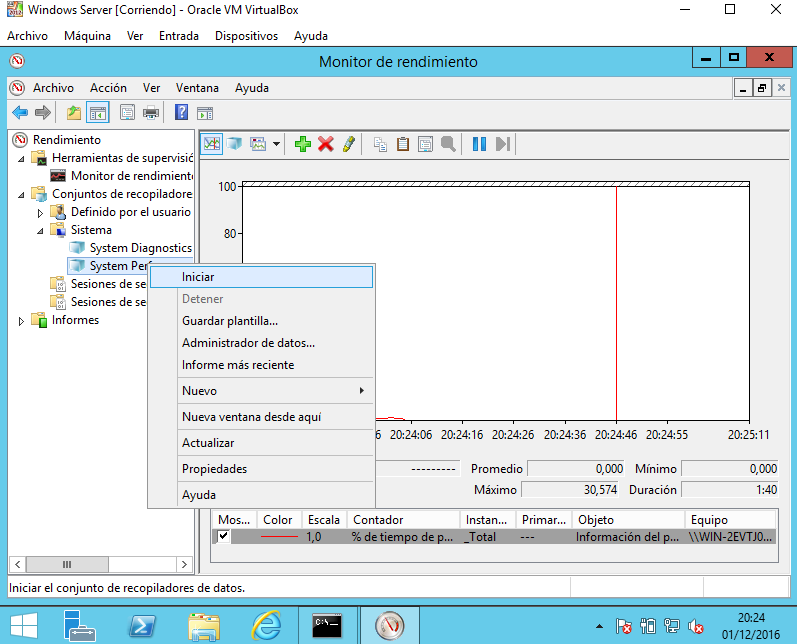
\includegraphics[scale=0.6]{figuras/figura6.png} 
	\caption{Ventana principal del Monitor de rendimiento de Windows} 
	\label{fig:figura6}
\end{figure}

Cuando acaba la ejecución aparece un nuevo informe en la pestaña \textbf{Informes} en el mismo panel actual.
\\

Para obtener la información basta con pulsar sobre éste y aparecerá un desglose con diferentes pestañas clasificadas según el tipo de información, como aparece en la Figura \ref{fig:figura7-1}

\begin{figure}[H] %con el [H] le obligamos a situar aquí la figura
	\centering
	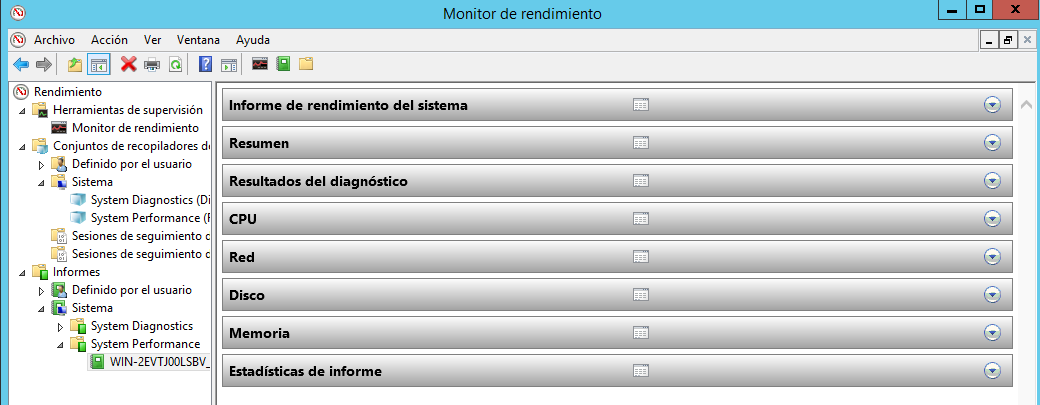
\includegraphics[scale=0.6]{figuras/figura7-1.png} 
	\caption{Ejecución del \textbf{System Performance}} 
	\label{fig:figura7-1}
\end{figure}

En la Figura \ref{fig:figura7-2} aparecen abiertas algunas pestañas importantes: 

\begin{itemize}
	\item El \textbf{informe de rendimiento de sistema} en el que se muestra el equipo, la fecha y la duración de la ejecución.
	
	\item Un \textbf{resumen}, en el que aparecen diferentes evaluaciones importantes como son el uso de memoria, disco y CPU. Se trata de una información no detallada pero que puede resultar muy útil para informes rápidos.
	
	\item El \textbf{rendimiento}, en el que se presenta la información general de recursos de la CPU, Red, Disco y Memoria con un mínimo detalles.
\end{itemize}

\begin{figure}[H] %con el [H] le obligamos a situar aquí la figura
	\centering
	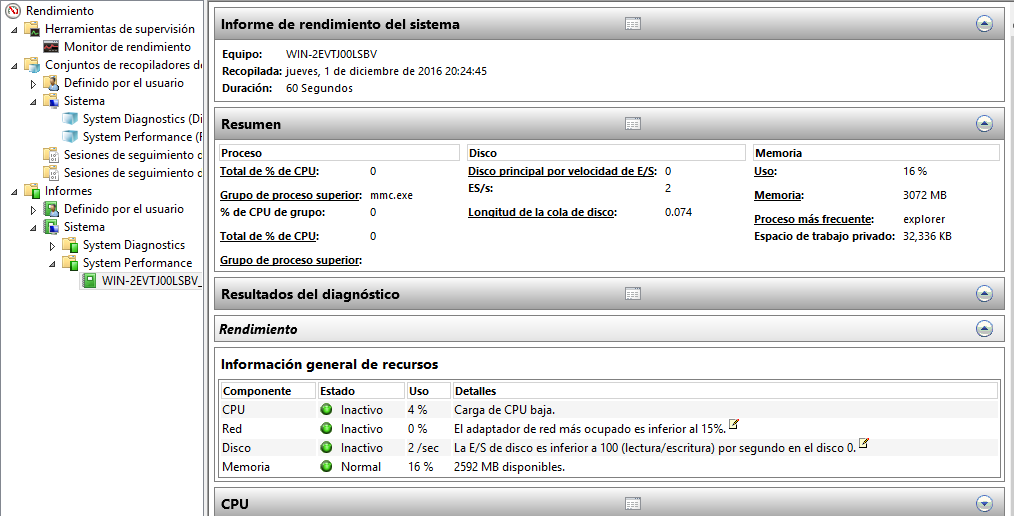
\includegraphics[scale=0.5]{figuras/figura7-2.png} 
	\caption{Ejecución del \textbf{System Performance}} 
	\label{fig:figura7-2}
\end{figure}

El resto de pestañas ya sí que ofrecen unas evaluaciones bastante detalladas sobre los distintos componentes del sistema antes mencionados.
\\

En la Figura \ref{fig:figura8} se ven dichas evaluaciones que, por ejemplo, permiten conocer los bytes enviados/recibidos desde una interfaz de Red específica del sistema; así como el tiempo medio de lectura/escritura en un disco duro físico, entre muchas otras.

\begin{figure}[H] %con el [H] le obligamos a situar aquí la figura
	\centering
	\includegraphics[scale=0.55]{figuras/figura8.png} 
	\caption{Pestañas de información detallada de \textbf{System Performance}} 
	\label{fig:figura8}
\end{figure}

\newpage



%----------------------------------------------------------------------------------------
%	Cuestión 5
%----------------------------------------------------------------------------------------

\section{Cuestión 5}
\subsection{Cree un recopilador de datos definido por el usuario (modo
	avanzado) que incluya tanto el contador de rendimiento como los datos de
	seguimiento}

	Para comenzar lo primero es abrir la herramienta \textbf{Monitor de rendimiento}. Una vez ahí, hay que situarse en el panel lateral izquierdo de la herramienta y pulsar sobre \textbf{Conjuntos de recopiladores} $ \rightarrow $ \textbf{Definido por el usuario}.
	Sobre éste último hacer clic con el botón derecho del ratón y, a continuación, \textbf{Nuevo} $ \rightarrow $ \textbf{Conjunto de recopiladores de datos}.
	\\
	
	La Figura \ref{fig:figura9} muestra dicho proceso con la ayuda de unas flechas rojas adicionales.
	
	\begin{figure}[H] %con el [H] le obligamos a situar aquí la figura
		\centering
		\includegraphics[scale=0.7]{figuras/figura9.png} 
		\caption{Nuevo conjunto de recopiladores} 
		\label{fig:figura9}
	\end{figure}

	La siguiente ventana que aparece solicita que se le asigne el nombre que va a tener el recopilador y el modo en el que se va a crear. 
	
	En este caso se pulsara la pestaña \textbf{Crear manualmente (avanzado)} tal y como se ve en la Figura \ref{fig:figura10}.
	
	\begin{figure}[H] %con el [H] le obligamos a situar aquí la figura
		\centering
		\includegraphics[scale=0.55]{figuras/figura10.png} 
		\caption{Nombre y modo de creación del conjunto} 
		\label{fig:figura10}
	\end{figure}
	
	Ahora hay que elegir qué tipo de datos se desea incluir. En el enunciado de este ejercicio se piden los siguientes:	
	\begin{itemize}
		\item [$ \checkmark $] Contador de rendimiento 
		\item [$ \checkmark $] Datos de	seguimiento
	\end{itemize}
	
	Se pulsan las pestañas mencionadas anteriormente  (como enseña la Figura \ref{fig:figura11}) y se hace clic en siguiente.
	
	\begin{figure}[H] %con el [H] le obligamos a situar aquí la figura
		\centering
		\includegraphics[scale=0.55]{figuras/figura11.png} 
		\caption{Tipos de datos a incluir en el recopilador} 
		\label{fig:figura11}
	\end{figure}
	
	A continuación aparecerá una nueva ventana en la que habrá que espeficcar qué contadores de rendimientos se desea registrar.
	
	Para ello habrá que pulsar sobre \textbf{Agregar} (marcado con una flecha roja en la Figura \ref{fig:figura12})
	
	\begin{figure}[H] %con el [H] le obligamos a situar aquí la figura
		\centering
		\includegraphics[scale=0.7]{figuras/figura12.png} 
		\caption{Qué contadores de rendimiento registrar} 
		\label{fig:figura12}
	\end{figure}
	
	Después de pulsar \textbf{Agregar} habrá que incluir los contenedores que se deseen en la lista. 
	
	En la parte izquierda de la ventana aparece un panel con todos los contadores disponibles (en este caso en el \textbf{Equipo local}). Se buscarán los tres que se piden en el enunciado:
	
	\begin{itemize}
		\item [$ \checkmark $] Procesador 
		\item [$ \checkmark $] Proceso
		\item [$ \checkmark $] Servicio web
	\end{itemize}

	Cada vez que se seleccione un contenedor, hay que elegir también las instancias del objeto (\textbf{<Todas las instancias>}) y, de forma seguida, habrá que pulsar sobre el botón \textbf{Agregar} que se encontrará más abajo de la misma ventana.
	
	\begin{figure}[H] %con el [H] le obligamos a situar aquí la figura
		\centering
		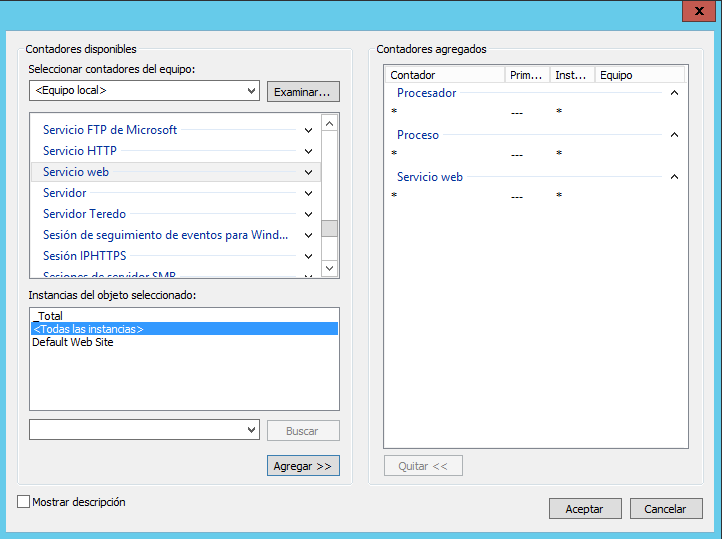
\includegraphics[scale=0.55]{figuras/figura13.png} 
		\caption{Agregar contenedores} 
		\label{fig:figura13}
	\end{figure}
	
	Una vez agregados dichos contenedores deben de aparecer en el panel de la derecha de la ventana \textbf{Contenedores agregados}, tal y como muestra la Figura \ref{fig:figura13}.
	
	\begin{figure}[H] %con el [H] le obligamos a situar aquí la figura
		\centering
		\includegraphics[scale=0.55]{figuras/figura14.png} 
		\caption{Contadores de rendimiento para registrar} 
		\label{fig:figura14}
	\end{figure}
	
	Cerrada la ventana anterior, vuelve a aparecer la misma en la que se encontraba el proceso pero, esta vez, con los contadores de rendimiento incluidos en el registro (Figura \ref{fig:figura14})
	\\
	
	En ésta solo queda asegurar que el intervalo de muestra sea de 15 segundos que puede verse en la Figura \ref{fig:figura14}, tal y como pide el enunciado del ejercicio.
	
	\begin{figure}[H] %con el [H] le obligamos a situar aquí la figura
		\centering
		\includegraphics[scale=0.6]{figuras/figura15.png} 
		\caption{Directorio de destino del informe} 
		\label{fig:figura15}
	\end{figure}
	
	Para finalizar el proceso de creación del conjunto de recopiladores solo queda especificar el directorio donde se van a almacenar los resultados, en el que en este caso sera \textbf{Escritorio\textbackslash logs}. Si la carpeta no existe, se creará como aparece en la Figura \ref{fig:figura15}.

	\begin{figure}[H] %con el [H] le obligamos a situar aquí la figura
		\centering
		\includegraphics[scale=0.55]{figuras/figura16.png} 
		\caption{Finalizado del proceso de creación de recopiladores} 
		\label{fig:figura16}
	\end{figure}

	En la última ventana (como la de la Figura \ref{fig:figura16}) que aparece hay que especificar que se desea que se inicie ahora el conjunto de recopiladores y \textbf{Finalizar}.
	\\
	
	Ya se puede comprobar cómo se encuentra \textbf{activo} el recopilador recientemente creado. En la Figura \ref{fig:figura17} puede verse que el funcionamiento parece correcto.
	
	\begin{figure}[H] %con el [H] le obligamos a situar aquí la figura
		\centering
		\includegraphics[scale=0.8]{figuras/figura17.png} 
		\caption{Recopilador definido activo} 
		\label{fig:figura17}
	\end{figure}
	
	Para poder visualizar los resultados hay que detener el recopilador y pulsar sobre el informe que se ha creado. Se tienen dos opciones:
	
	\begin{enumerate}
		\item Desde el directorio que se le ha especificado en las propiedades (Figura \ref{fig:figura19})		
			\begin{figure}[H]
				\centering
				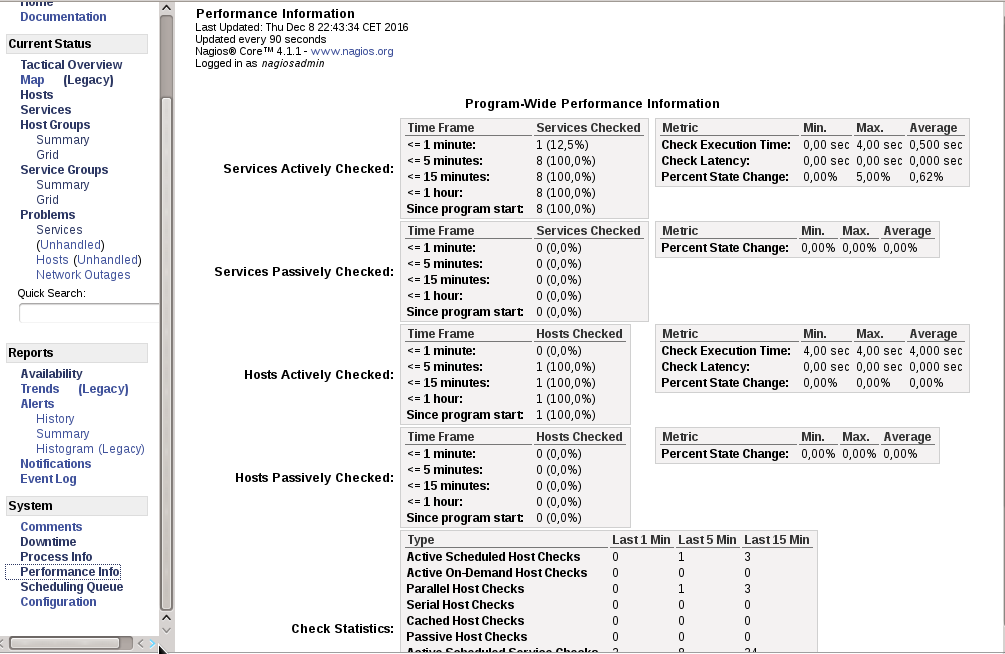
\includegraphics[scale=0.9]{figuras/figura19.png} 
				\caption{Directorio de almacenamiento de resultados} 
				\label{fig:figura19}
			\end{figure}
\newpage

		\item Desde el Monitor de rendimiento, Figura \ref{fig:figura21},
		\textbf{Panel izquierdo Rendimiento} $ \rightarrow $ \textbf{Informes} $ \rightarrow $ \textbf{Definido por el usuario} $ \rightarrow $ \textbf{Nombre del recopilador}
			\begin{figure}[H]
				\centering
				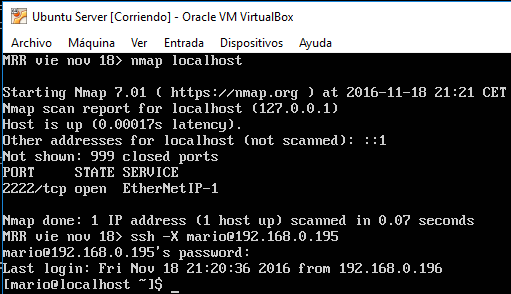
\includegraphics[scale=0.7]{figuras/figura21.png} 
				\caption{Informe del recopilador en Monitor de rendimiento} 
				\label{fig:figura21}
			\end{figure}
	\end{enumerate}	
	
\newpage

%----------------------------------------------------------------------------------------
%	Cuestión 6
%----------------------------------------------------------------------------------------

\section{Cuestión 6}
\subsection{Visite la web del proyecto y acceda a la demo que
	proporcionan (\url{http://demo.munin-monitoring.org/}) donde se muestra cómo
	monitorizar un servidor. Monitorice varios parámetros y haga capturas de
	pantalla de lo que está mostrando comentando qué observa.}

La demo que proporciona Munin permite ver una gran cantidad de gráficas relativas a distintas categorías. En este caso se han elegido las necesarias para mostrar su funcionamiento.
\\

Cada monitorización muestra cuatro gráficas: diaria, semanal, mensual y anual. Además, también aparecen valores actuales, mínimos, medios y máximos.
En la sección de disco se puede ver las entradas y salidas por dispositivo que, en el caso de este servidor, contiene solo un disco así que solo muestra una linea.
\\

En la Figura \ref{fig:figura61} aparece el número de operaciones IO por segundo (en azul) y el tamaño medio de estas solicitudes (en amarillo). Los datos son de los días lunes, martes y jueves.

\begin{figure}[H]
	\centering
	\includegraphics[scale=0.65]{figuras/ejercicio6/figura1.png} 
	\caption{IOs for /dev/sda \cite{enlace5}} 
	\label{fig:figura61}
\end{figure}

\newpage

La Figura \ref{fig:figura62} muestra memoria usada por el sistema de ayer a hoy. En la gráfica aparecen los resultados obtenidos a través del uso de aplicaciones, buffers, caché, tablas de paginación, uso de swap...
\\

Aparecen cuatro columnas con la ocupación de cada tipo de uso divididas por un mínimo y un máximo, así como la media entre ellas.

\begin{figure}[H]
	\centering
	\includegraphics[scale=1]{figuras/ejercicio6/figura2.png} 
	\caption{Uso de memoria física \cite{enlace5}} 
	\label{fig:figura62}
\end{figure}

La siguiente Figura (Figura \ref{fig:figura63}) presenta los resultados que se han obtenido por la carga media del sistema desde ayer a hoy.
\\

Aparecen tres medidas distintas en la gráfica: de cada minuto, de cada 5 minutos y de cada 15 minutos, clasificadas también en las cuatro columnas anteriormente mencionadas.
\\

Que se hagan esas tres medidas diferentes es indispensable para que pueda apreciarse resultados claros en la carga diaria. Basta con comparar los resultados obtenidos cada 1 min con los de 15 minutos: en los de cada 15 minutos los cambios en la carga son inapreciables, mientras que en el contrario cada medida dista en gran cantidad con respecto a la anterior.

\begin{figure}[H]
	\centering
	\includegraphics[scale=1]{figuras/ejercicio6/figura3.png} 
	\caption{Load average \cite{enlace6}} 
	\label{fig:figura63}
\end{figure}

La gráfica siguiente, la de la Figura \ref{fig:figura64}, muestra el número para cada tipo de proceso que se ha ejecutado en el sistema de ayer hasta hoy.
\\

La mayor parte de los procesos han estado dormidos casi todo el tiempo en el que se han tomado los resultados. Hay una mínima parte en el que sí se ha estado activo algún proceso de forma ininterrumpida.

\begin{figure}[H]
	\centering
	\includegraphics[scale=1]{figuras/ejercicio6/figura4.png} 
	\caption{Procesos \cite{enlace7}} 
	\label{fig:figura64}
\end{figure}

\newpage

%----------------------------------------------------------------------------------------
%	Cuestión 7
%----------------------------------------------------------------------------------------

\section{Cuestión 7}
\subsection{Escriba un breve resumen sobre alguno de los artículos donde
	se muestra el uso de strace o busque otro y coméntelo}

\textbf{Lee Latham} en el blog web \textbf{Softlayer} \cite{enlace8}, explica el funcionamiento bastante detallado de \textbf{strace}. Segun él, strace sirve para observar las llamadas al sistema que hace un ejecutable. 
\\

Se trata de una herramienta que puede ayudar ante una situación en la que un ejecutable termina su ejecución sin saber por qué y, a pesar de ello, no aparece rastros de esta ejecución fallida en ningún registro o, por el contrario, no es útil la información que proporciona.
\\

En el blog, además, se hace un ejemplo de utilización de strace: 

Primero el usuario se identifica como \textbf{root} y crea un nuevo archivo llamado \textbf{test.txt}.
A continuación, se ejecuta \textbf{strace cat test.txt} y el programa retorna todas las llamadas al sistema. Además, se realiza un \textbf{open de test.txt} y un read del contenido, entre otras cosas.
\\

Después, se realiza un ejemplo real mediante \textbf{apache} para conocer el paredero en el que se van a escribir sus logs.
Para ello, lo que se hace es ejecutar strace con el reinicio del servicio \textbf{httpd}, escogiendo sólo las llamadas
al sistema de open.

En esta ocasión lo que se muestra son las llamadas que se producen para abrir los archivos de registro al iniciar el servicio y, posteriormente, conocer dónde se guardan los registros de dicho servicio.

\newpage

%----------------------------------------------------------------------------------------
%	Cuestión 8
%----------------------------------------------------------------------------------------

\section{Cuestión 8}
\subsection{Escriba un script en Python o PHP}
	\lstinputlisting[style=payt]{fuentes/sshPython.py}

	El script lo que hace es cambiar la linea del fichero de configuración de ssh (\textbf{/etc/ssh/sshd\_config}) en la que se especifica el puerto por el que funciona el servicio.
	\\
	
	El puerto nuevo será un número pasado como argumento y, por supuesto, la ejecución del script debe realizarse con \textbf{permisos root} para su correcta ejecución.
	\\
	
	En la Figura \ref{fig:figura81} se muestra un ejemplo de su ejecución en una máquina de Ubuntu. Primero se comprueba cuál es el puerto actual, a continuación se ejecuta el script y por último se comprueba de nuevo el fichero de configuración para ver si se ha cambiado correctamente.
	
	\begin{figure}[H]
		\centering
		\includegraphics[scale=0.8]{figuras/ejercicio8/figura1.png} 
		\caption{Prueba de ejecución de script en Python } 
		\label{fig:figura81}
	\end{figure}
	
\subsection{Analice el comportamiento del script
	usando el profiler presentado}

Se va a utilizar el profiler \textbf{cProfile} \cite{enlace9}, que es el recomendado para la mayoría de usuarios. Para poder invocarlo hay que realizar una de estas dos acciones:

\begin{enumerate}
	\item Añadir al script de python las siguientes lineas:
\begin{lstlisting}[style=cmas]
import cProfile
import re
cProfile.run('re.compile("foo|bar")')
\end{lstlisting}
		
	\item Ejecutar la siguiente orden desde la linea de comandos:
\begin{lstlisting}[style=fich]
$ python -m cprofile sshPython.py
\end{lstlisting}
\end{enumerate}

En este caso se ha utilizado, por comodidad, la primera opción.
\\

Ahora para su funcionamiento, basta con realizar la ejecución del script y ya de forma automática lo hace también el profiler.

En la Figura \ref{fig:figura82} aparece la ejecución del script junto con el profiler y el desglose de los resultados que se han obtenido.
En este caso, dado el poco conocimiento que tengo del tema, los resultados son bastante desconocidos. Es por ello que buscando información sobre cómo interpretar estos resultados encontré una herramienta que hace dicha interpretación algo más $ " $entendible$ " $ por medio de representaciones gráficas, por ejemplo.

\begin{figure}[H]
	\centering
	\includegraphics[scale=0.6]{figuras/ejercicio8/figura2.png} 
	\caption{Primera aproximación de ejecución del profiler} 
	\label{fig:figura82}
\end{figure}

Esta herramienta se llama \textbf{KCacheGrind} \cite{enlace10} en la que se encuentra la opción \textbf{pyprof2calltree} que lo que hace es convertir un archivo con un volcado de datos del profiler en uno compatible para si mismo, para su posterior representación en la aplicación.
\\

Por tanto, se instaló la herramienta por medio de la orden:
\begin{lstlisting}[style=fich]
$ sudo apt-get install kcachegrind
\end{lstlisting}


Hubo un problema a la hora de ejecutar \textbf{pyprof2calltree}, ya que ésta no se encontraba dentro de la herramienta y no encontré un comando para instalarla mediante \textbf{apt}.
Busqué el paquete y lo descargué desde su página (\url{https://pypi.python.org/pypi/pyprof2calltree/}). \\

Lo que se descarga es un fichero en python, por lo que para ejecutarla se debe de hacer como un script cualquiera de python con la peculiaridad de que debe de tener unos argumentos específicos, que son:
\begin{lstlisting}[style=fich]
$ pyprof2calltree.py [-k] [-o output\_file\_path] [-i input\_file\_path] [-r scriptfile [args]]
\end{lstlisting}

Una vez instalada la herramienta con todos sus componentes necesarios ya solo falta la parte más importante: el archivo con el volcado de datos.
Para ello basca con completar la linea donde se escribe la función run del cProfile con el nombre del archivo de salida. En este caso, la linea 7 del script que antes de la modificación era:

\begin{lstlisting}[style=fich]
cProfile.run('re.compile("foo|bar")')
\end{lstlisting}

Y, posteriormente a la modificación:

\begin{lstlisting}[style=fich]
cProfile.run('re.compile("foo|bar")', 'salida.cprof')
\end{lstlisting}


A continuación se procede a la conversión del fichero con el volcado de los resultados (que previamente se han obtenido al ejecutar el script personal), para ello se ejecuta la siguiente orden, tal y como muestra la Figura \ref{fig:figura83}:

\begin{lstlisting}[style=fich]
python pyprof2calltree.py -k -i salida.cprof
\end{lstlisting}

\begin{figure}[H]
	\centering
	\includegraphics[scale=0.8]{figuras/ejercicio8/figura3.png} 
	\caption{Presentación de los datos obtenidos con Kcachegrind} 
	\label{fig:figura83}
\end{figure}

\newpage

Finalmente, ya sí que se han obtenido un volcado de los resultados del profiler mejor representados. Basta con observar la Figura \ref{fig:figura84}.

\begin{figure}[H]
	\centering
	\includegraphics[scale=0.8]{figuras/ejercicio8/figura4.png} 
	\caption{Primera aproximación de ejecución del profiler} 
	\label{fig:figura84}
\end{figure}

La Figura \ref{fig:figura85} aparece una gráfica en forma de árbol obtenida también en Kcachegrind (desde \textbf{Call graph}) en el que se presenta el tiempo que gastan las llamadas al sistema en una ejecución concreta, así como la relación coexistente entre cada llamada.

\begin{figure}[H]
	\centering
	\includegraphics[scale=0.8]{figuras/ejercicio8/figura5.png} 
	\caption{Representación de la organización del tiempo de las llamadas} 
	\label{fig:figura85}
\end{figure}

En ésta se puede ver cómo la función \textbf{module} (llamada 0) y a compile son la que más tiempo requieren en este script mientras que, por el contrario, la llamada \textbf{get} (llamada 8) es la que menos.
\newpage

%----------------------------------------------------------------------------------------
%	Cuestión 9
%----------------------------------------------------------------------------------------

\section{Cuestión 9}
\subsection{Acceda a la consola mysql (o a través de phpMyAdmin) y
	muestre el resultado de mostrar el ”profile” de una consulta (la creación de
	la BD y la consulta la puede hacer libremente)}

En este caso se ha realizado el ejercicio a través de la \textbf{consola mysql}.\\

En primer lugar, una vez en la consola MariaDB o Mysql, se crea la base de datos para poder hacer la prueba mediante la orden $ ' $\textbf{CREATE DATABASE nombre\_database ;} $ ' $ (sin las comillas).\\

A continuación, con la orden $ ' $\textbf{USE nombre\_database ;} $ ' $ se accede a la database creada para poder trabajar sobre ella. \\

Todo este proceso anterior puede verse en la Figura \ref{fig:figura91}.

\begin{figure}[H]
	\centering
	\includegraphics[scale=0.9]{figuras/ejercicio9/figura1.png} 
	\caption{Creación de una nueva base de datos en Mysql} 
	\label{fig:figura91}
\end{figure}

Ahora, ya se pueden crear tablas sobre la base de datos creada. Se crearán dos como ejemplo: una llamada pueblo y otra llamada país a través de la orden \textbf{CREATE TABLE nombre\_tabla (nombre\_column tipo\_column) ;} mostrándolas seguidamente con \textbf{SHOW TABLES ;} como aparece en la 
Figura \ref{fig:figura92}.

\begin{figure}[H]
	\centering
	\includegraphics[scale=0.9]{figuras/ejercicio9/figura2.png} 
	\caption{Creación de tablas en Mysql} 
	\label{fig:figura92}
\end{figure}

Una vez las tablas están creadas, hay que comprobar si el profiler se encuentra en funcionamiento. Para ello basta con ejecutar la orden \textbf{SELECT $ @ $$ @ $profiling ;} y ver si su valor es \textbf{uno} (si es cero es que no está activo).\\

Como se muestra en la Figura \ref{fig:figura93} tras la primera comprobación su valor es \textbf{cero}. Para cambiarlo se utiliza la orden \textbf{SET profiling=1 ;}, como aparece en esta misma figura.

\begin{figure}[H]
	\centering
	\includegraphics[scale=1]{figuras/ejercicio9/figura3.png} 
	\caption{Activación del profiler en Mysql} 
	\label{fig:figura93}
\end{figure}

Para poder obtener resultados con el profiler hay que realizar alguna consulta \cite{enlace11}. En la Figura \ref{fig:figura94} presenta la consulta que se ha hecho en este caso (con la orden \textbf{SELECT} para seleccionar datos de una tabla) y los resultados que se han obtenido después con el profiler con la orden \textbf{SHOW PROFILES ;} con la que se muestra información detallada acerca de \textbf{un solo estado}, la declaración ejecutada más recientemente. 

\begin{figure}[H]
	\centering
	\includegraphics[scale=0.9]{figuras/ejercicio9/figura4.png} 
	\caption{Utilización profiler en Mysql} 
	\label{fig:figura94}
\end{figure}

Por otro lado, hay otra orden en la que en cambio aparece una \textbf{lista} de las declaraciones más recientes enviadas al servidor. Ésta es \textbf{SHOW PROFILE ;} \cite{enlace11} y puede verse un ejemplo de uso en la Figura \ref{fig:figura95}.

\begin{figure}[H]
	\centering
	\includegraphics[scale=0.8]{figuras/ejercicio9/figura5.png} 
	\caption{Utilización profiler en Mysql} 
	\label{fig:figura95}
\end{figure}

Para especificar sobre qué consulta se quiere ver el registro, hay que añadir a \textbf{SHOW PROFILE} el operador \textbf{FOR QUERY Query\_ID} (ver Figura \ref{fig:figura96}), donde \textbf{Query\_ID} es el ID de consulta tal y como se ha listado en \textbf{SHOW PROFILES ;}\\

\begin{figure}[H]
	\centering
	\includegraphics[scale=0.9]{figuras/ejercicio9/figura7.png} 
	\caption{Utilización profiler en Mysql} 
	\label{fig:figura96}
\end{figure}

Sin embargo, si lo que se quiere es que se muestre un tipo concreto de registro se le puede especificar justo antes del operador \textbf{FOR}, como en el caso de la Figura \ref{fig:figura96}, donde se le ha especificado que muestre los datos de uso de \textbf{memoria}.


\newpage

%----------------------------------------------------------------------------------------
%	Cuestión Opcional 2
%----------------------------------------------------------------------------------------

\section{Cuestión opcional 2}
\subsection{Instale Nagios en su sistema (el que prefiera)
	documentando el proceso y muestre el resultado de la monitorización de su
	sistema comentando qué aparece}

Se va a proceder a instalar \textbf{Nagios Core} en Centos 7. \cite{enlace12}

\begin{itemize}
	\item Instalación de los paquetes necesarios (Figura \ref{fig:figura121}) para satisfacer las dependencias de la herramienta mediante la orden:
\begin{lstlisting}[style=fich]
> sudo yum install gcc glibc glibc-common gd gd-devel make net-snmp openssl-devel xinetd unzip
\end{lstlisting}	
	\begin{figure}[H]
		\centering
		\includegraphics[scale=0.68]{figuras/ejercicio12/figura1.png} 
		\caption{Instalación de los paquetes necesarios para Nagios} 
		\label{fig:figura121}
	\end{figure}

	\item Creación de usuario y grupo (Figura \ref{fig:figura122}), para que se ejecute el proceso de Nagios, a través las órdenes:
\begin{lstlisting}[style=fich]
> sudo useradd nagios
> sudo groupadd nagcmd
> sudo usermod -a -G nagcmd nagios
> sudo usermod -a -G nagcmd apache
\end{lstlisting}
	
	\begin{figure}[H]
		\centering
		\includegraphics[scale=0.8]{figuras/ejercicio12/figura2.png} 
		\caption{Creación de usuario y grupo para Nagios} 
		\label{fig:figura122}
	\end{figure}
	
	\item Antes de comenzar nuestra instalación, se necesita inhabilitar \textbf{SELinux (Figura \ref{fig:figura123})}.
	Para ello basta con modificar una linea en el fichero \textbf{/etc/selinux/config}:
\begin{lstlisting}[style=fich]
SELINUX=disabled
\end{lstlisting}	
	\begin{figure}[H]
		\centering
		\includegraphics[scale=1]{figuras/ejercicio12/figura3.png} 
		\caption{Deshabilitación de SELinux} 
		\label{fig:figura123}
	\end{figure}

	\item Descarga de Nagios y sus plugins.
	Con las siguientes órdenes se descargará, como aparece en la Figura \ref{fig:figura124}, tanto la herramienta como los plugins necesarios para su funcionamiento:
\begin{lstlisting}[style=fich]
> cd /tmp
> wget https://assets.nagios.com/downloads/nagioscore/releases/nagios-4.1.1.tar.gz
> wget http://www.nagios-plugins.org/download/nagios-plugins-2.1.1.tar.gz
> tar zxf nagios-4.1.1.tar.gz
> tar zxf nagios-plugins-2.1.1.tar.gz
> cd nagios-4.1.1
\end{lstlisting}

	\begin{figure}[H]
		\centering
		\includegraphics[scale=1]{figuras/ejercicio12/figura4.png} 
		\caption{Descarga de Nagios y sus plugins} 
		\label{fig:figura124}
	\end{figure}

	\item Instalación de Nagios.
	Ahora que todos los archivos se han descomprimido es el momento de su compilación e instalación. Tal y como aparece en las Figuras \ref{fig:figura125}, \ref{fig:figura126},\ref{fig:figura127},\ref{fig:figura128}; se utilizan las siguientes órdenes:
\begin{lstlisting}[style=fich]
> ./configure --with-command-group=nagcmd
> make all
> make install
> make install-init
> make install-config
> make install-commandmode
> make install-webconf
\end{lstlisting}

	\begin{figure}[H]
		\centering
		\includegraphics[scale=1]{figuras/ejercicio12/figura7.png} 
		\caption{Instalación de Nagios} 
		\label{fig:figura125}
	\end{figure}
	\begin{figure}[H]
		\centering
		\includegraphics[scale=0.94]{figuras/ejercicio12/figura8.png} 
		\caption{Instalación de Nagios} 
		\label{fig:figura126}
	\end{figure}
	\begin{figure}[H]
		\centering
		\includegraphics[scale=0.94]{figuras/ejercicio12/figura9.png} 
		\caption{Instalación de Nagios} 
		\label{fig:figura127}
	\end{figure}
	\begin{figure}[H]
		\centering
		\includegraphics[scale=0.94]{figuras/ejercicio12/figura10.png} 
		\caption{Instalación de Nagios} 
		\label{fig:figura128}
	\end{figure}

	\item Creación de una contraseña de acceso a Nagios.
	Es necesario que se cree una contraseña vinculada a la cuenta \textbf{nagiosadmin} anteriormente creada para el acceso a la herramienta.
	En la Figura \ref{fig:figura130} se ve la ejecución de la siguiente orden, en la que se requiere y se completa una contraseña.
\begin{lstlisting}[style=fich]
> htpasswd -c /usr/local/nagios/etc/htpasswd.users nagiosadmin
\end{lstlisting}
	
	\begin{figure}[H]
		\centering
		\includegraphics[scale=1]{figuras/ejercicio12/figura11.png} 
		\caption{Creación de la contraseña de usuario para Nagios} 
		\label{fig:figura130}
	\end{figure}

	\item Instalación de los plugins necesarios para Nagios.
	Ahora que Nagios está instalado, se necesitan instalar los plugins (Figura \ref{fig:figura131}) para que pueda utilizarlos.
\begin{lstlisting}[style=fich]
> cd /tmp/nagios-plugins-2.1.1
> ./configure --with-nagios-user=nagios --with-nagios-group=nagios --with-openssl
> make all
> make install
\end{lstlisting}
	
	\begin{figure}[H]
		\centering
		\includegraphics[scale=1]{figuras/ejercicio12/figura12.png} 
		\caption{Instalación de los plugins necesarios para Nagios} 
		\label{fig:figura131}
	\end{figure}

\newpage

	\item Apertura de los puertos para Nagios.
	Hay que asegurar que los puertos de conexión que utiliza la herramienta (\textbf{80/tcp}) se encuentran abiertos. Si no es así, como en este caso, hay que abrirlos mediante las órdenes (Figura \ref{fig:figura132}) para que pueda utilizarlos.
\begin{lstlisting}[style=fich]
> firewall-cmd --zone=public --add-port=80/tcp --permanent
> firewall-cmd --reload
\end{lstlisting}
	
	\begin{figure}[H]
		\centering
		\includegraphics[scale=1]{figuras/ejercicio12/figura15.png} 
		\caption{Apertura de los puertos para Nagios} 
		\label{fig:figura132}
	\end{figure}

	\item Inicio de Nagios.
	Si todo el proceso realizado hasta ahora ha sido correcto, solo queda iniciar el servicio para su utilización, como se ve en la Figura \ref{fig:figura133}, con las siguientes órdenes:
\begin{lstlisting}[style=fich]
> service httpd start
> service nagios start
\end{lstlisting}
	
	\begin{figure}[H]
		\centering
		\includegraphics[scale=1]{figuras/ejercicio12/figura14.png} 
		\caption{Inicio de Nagios} 
		\label{fig:figura133}
	\end{figure}
\end{itemize}

\newpage

Una vez terminado el proceso de instalación, se comprobará si funciona todo correctamente. Para ello hay que acceder al navegador e ir a la dirección \textbf{http://localhost/nagios/}.

A continuación se requerirá un login (Figura \ref{fig:figura134}), que se completará con los datos que se han especificado en el proceso de instalación. 
\begin{figure}[H]
	\centering
	\includegraphics[scale=0.67]{figuras/ejercicio12/figura16.png} 
	\caption{Login en Nagios} 
	\label{fig:figura134}
\end{figure}

Si el login es correcto, por fin aparecerá la pantalla principal de Nagios igual que en la Figura \ref{fig:figura135}.

\begin{figure}[H]
	\centering
	\includegraphics[scale=0.6]{figuras/ejercicio12/figura17.png} 
	\caption{Pantalla principal de Nagios} 
	\label{fig:figura135}
\end{figure}

Ahora ya se puede obtener información de monitoreo con Nagios. Si se pulsa en el panel izquierdo sobre \textbf{Tactical Overview} puede verse
un resumen bastante detallado del sistema.

En éste, que es algo como la Figura \ref{fig:figura136}, se muestra las funciones del monitoreo, el estado de los servicios, los dispositivos conectados, el rendimiento del monitoreo... etc

\begin{figure}[H]
	\centering
	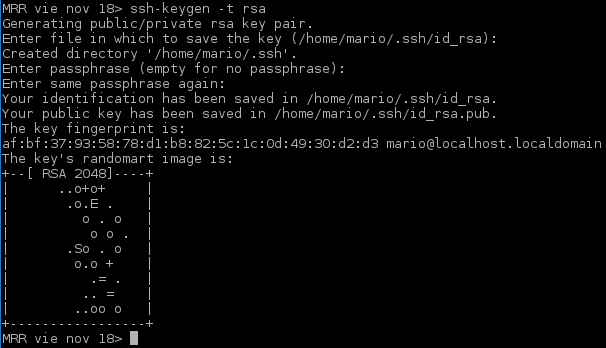
\includegraphics[scale=0.48]{figuras/ejercicio12/figura18.png} 
	\caption{Tactical Overview Nagios} 
	\label{fig:figura136}
\end{figure}

En la Figura \ref{fig:figura137} se muestran los detalles del estado del servicio para todos los hosts en la que, por ejemplo, muestra un aviso en el servicio HTTP ya que antes de acceder a esta herramienta he puesto mal el login y es lo que ha registrado.

\begin{figure}[H]
	\centering
	\includegraphics[scale=0.6]{figuras/ejercicio12/figura20.png} 
	\caption{Estados de los servicios Nagios} 
	\label{fig:figura137}
\end{figure}

La Figura \ref{fig:figura138} presenta los resultados obtenidos a través de la información del rendimiento del sistema, desde la opción \textbf{System}$ \rightarrow $\textbf{Performance info}.

\begin{figure}[H]
	\centering
	\includegraphics[scale=0.6]{figuras/ejercicio12/figura19.png} 
	\caption{Informacion de rendimiento en Nagios} 
	\label{fig:figura138}
\end{figure}

Éstos se muestran en tablas, clasificados en distintos periodos de tiempo para cada servicio verificado. Aparecen resultados de servicios y hosts activos/pasivos, así como las estadísticas resumidas en una tabla distinta.

\newpage

%----------------------------------------------------------------------------------------
%	Referencias
%----------------------------------------------------------------------------------------
%------------------------------------------------

\bibliography{citas} %archivo citas.bib que contiene las entradas 
\bibliographystyle{plain} % hay varias formas de citar

\end{document}
